\subsection{Students}

A brief reminder of what some of the tasks a user is supposed to perform includes inputing student preferences and selecting skills.
These will be converted into integer equivalences to be used by our ILP when it is time to assign students to classes.
Students self input all of their information, but we allow admins to be able to edit this information when they see fit.
Our hope is the students know what they are capable of teaching which means knowing the skills and languages they possess along with the classes they would like to teach.

\subsubsection{Student Experience Interface}

\begin{figure}[!htb]
  \centering
  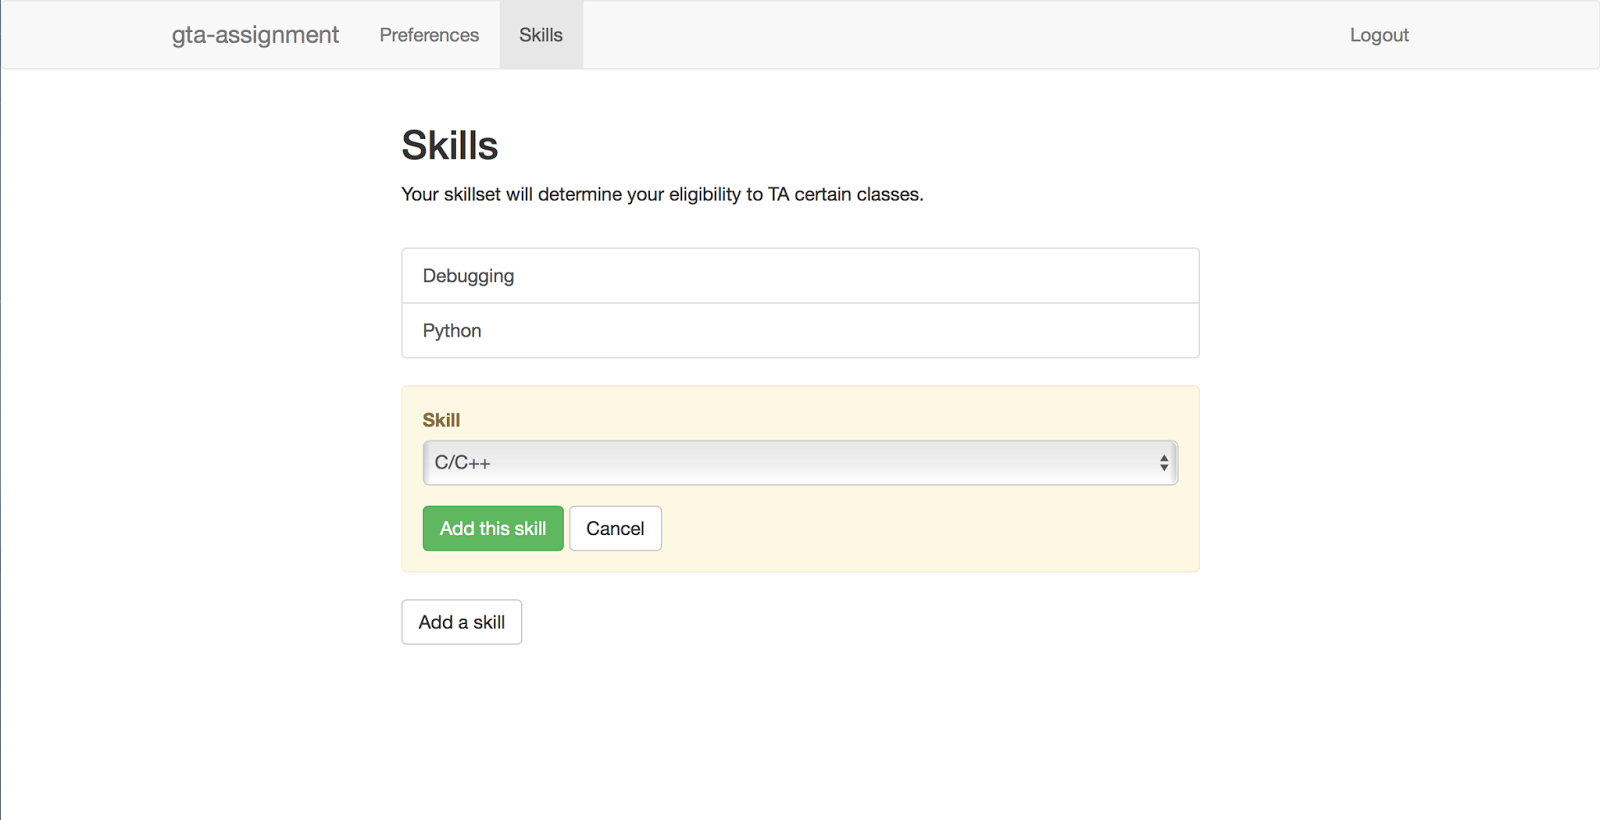
\includegraphics[width=0.75\linewidth]{images/student-experience-design.png}
  \caption{Mock Student Experience Interface}
\end{figure}
\begin{figure}[!htb]
  \centering
  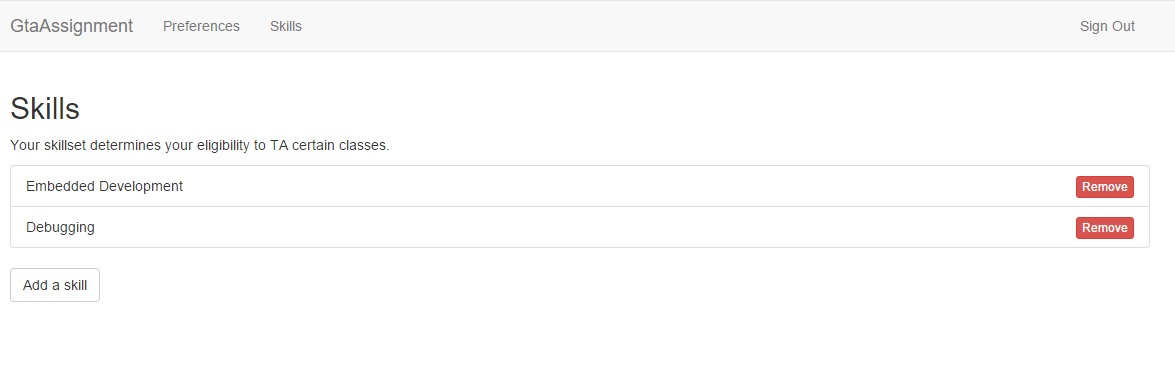
\includegraphics[width=0.75\linewidth]{images/student-experience-alpha.png}
  \caption{Alpha Student Experience Interface}
\end{figure}
\begin{figure}[!htb]
  \centering
  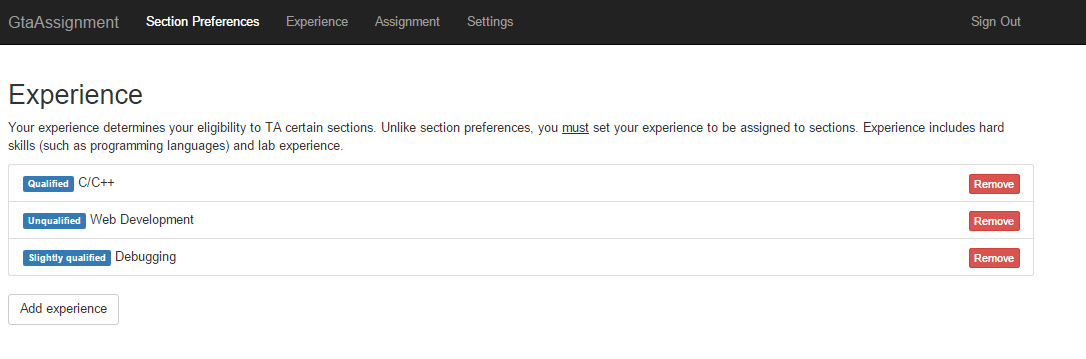
\includegraphics[width=0.75\linewidth]{images/student-experience-beta.png}
  \caption{Release Student Experience Interface}
\end{figure}

% \begin{figure}[!htb]
%   \centering
%   \minipage{0.5\textwidth}
%     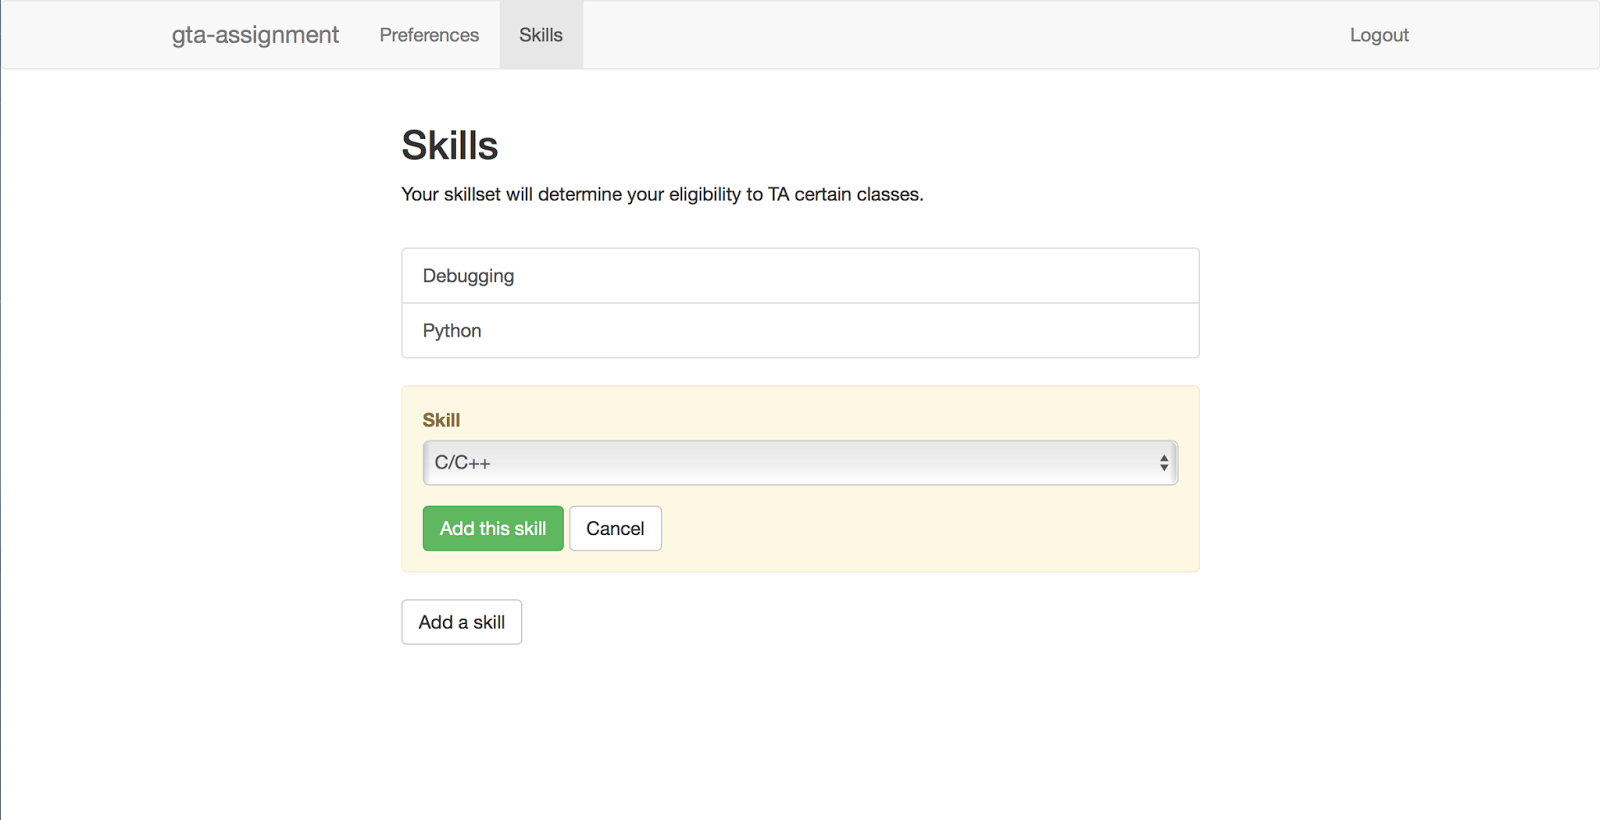
\includegraphics[width=\linewidth]{images/student-experience-design.png}
%     \caption{Mock Student Experience Interface}
%   \endminipage\hfill
%   \minipage{0.5\textwidth}
%     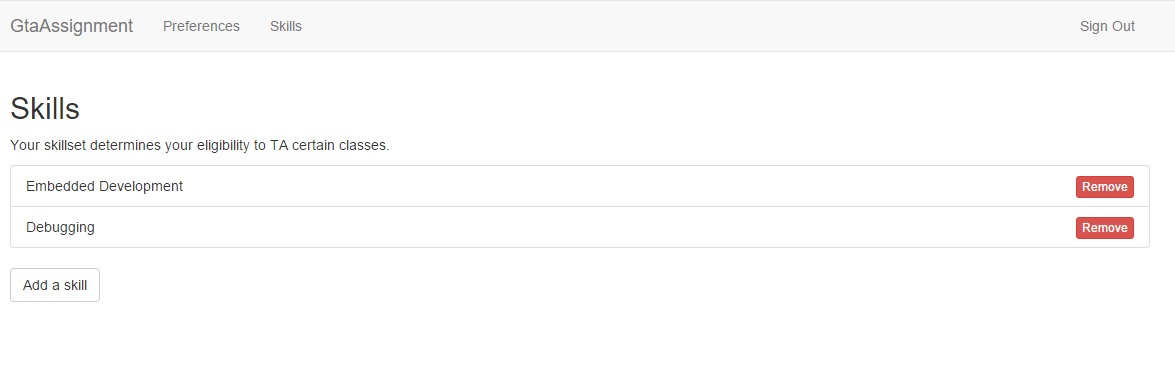
\includegraphics[width=\linewidth]{images/student-experience-alpha.png}
%     \caption{Alpha Student Experience Interface}
%   \endminipage\hfill
%   \minipage{0.5\textwidth}
%     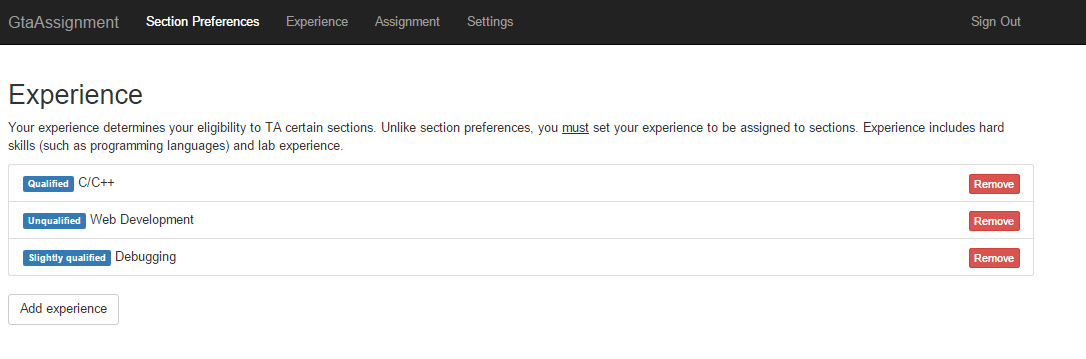
\includegraphics[width=\linewidth]{images/student-experience-beta.png}
%     \caption{Release Student Experience Interface}
%   \endminipage\hfill
% \end{figure}

This section hasn't changed much on the surface from what he had back in Fall - we added a few of sentences describing our project for those who had never used the site before.
The primary changes were on the backend.
After talking with our sponsor we felt that we should focus on combining skills and experience in one super section.
Skills acquired through school might have been acquired differently than a graduate student's experience outside of school yet, they both hold the same fundamental value within the ILP.

\begin{figure}[!htb]
   \centering
   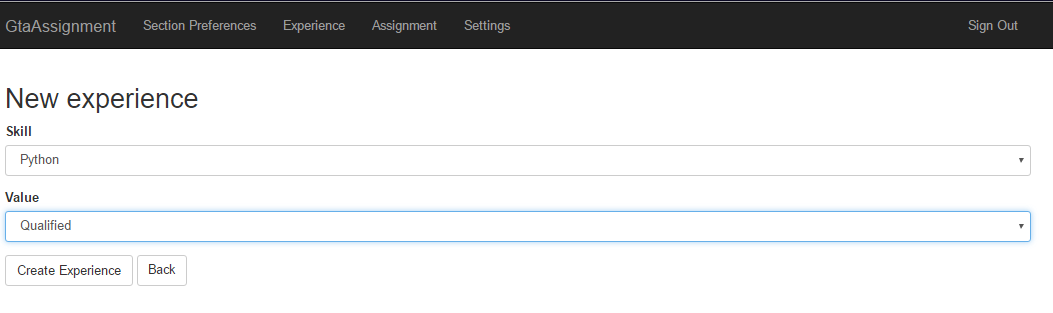
\includegraphics[width=0.75\textwidth]{images/student-new-experience-beta.png}
   \caption{How Students Add Experience From Pre-Defined List of Skills}\label{student-new-experience-beta}
\end{figure}

In Figure \ref{student-new-experience-beta}, one can see that the skill bar is a dropdown which has a list of predefined skills and experience.
With the help of our sponsor we came up with a default list that consists of skills such as python, C, C++, web development, debugging, and many more.
However, if an instructor doesn't see a skill they require, they can always add it via the instructor interface.
Each skill is associated with a student, for as long as they are a TA at Oregon State.
We allow students to select as many skills as they want.
The value that you see ranges from qualified, slightly qualified, to unqualified, where the default value are set to unqualified.
We are giving the power to the students to select the exact skills and experiences that they possess.
This selection is very important to us as it is programmed as a hard constraint in the ILP.
If a student does not have the right skills than they will not be eligible to teach the class.

\subsubsection{Student Preferences}

Student preferences are a key component of the ILP because the goal is to put students in classes they would want to teach.
Currently, we allow the students to select up to 5 classes that they favor or disfavor.
Almost as important as a class a student favors, what a student disfavors can be just as valuable.

\begin{figure}[!htb]
  \centering
  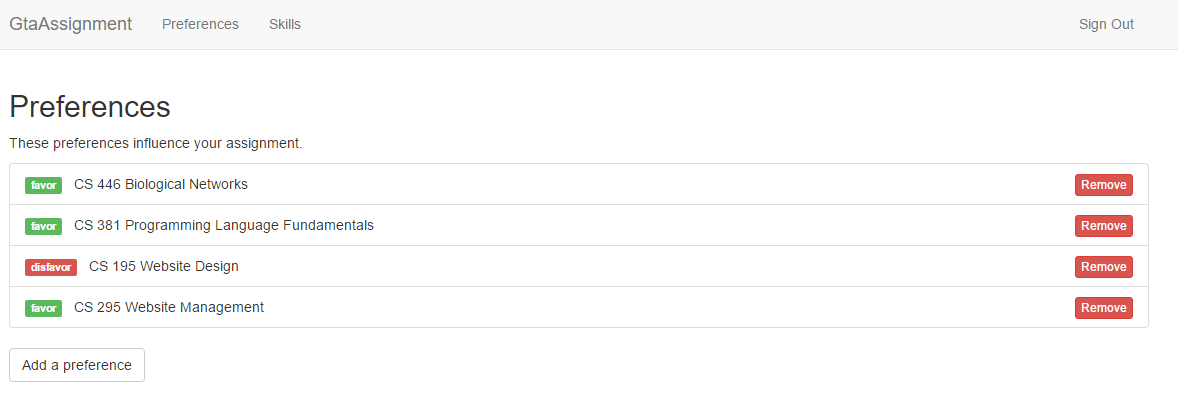
\includegraphics[width=0.75\linewidth]{images/student-preferences-alpha.png}
  \caption{Mock Student Preferences Interface}
\end{figure}
\begin{figure}[!htb]
  \centering
  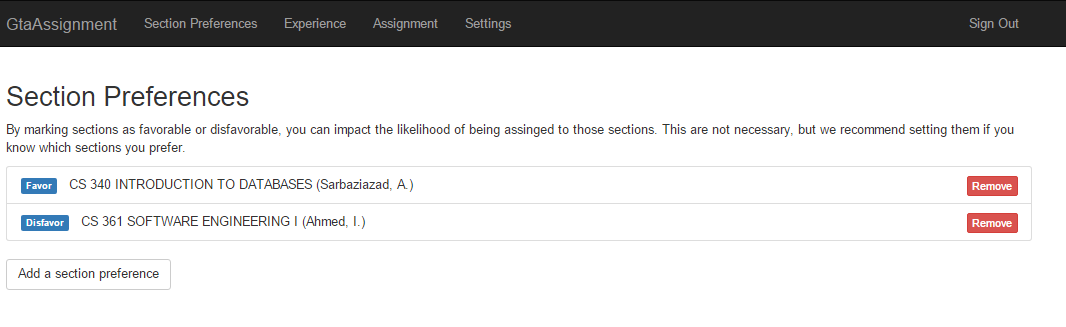
\includegraphics[width=0.75\linewidth]{images/student-preferences-beta.png}
  \caption{Release Student Preferences Interface}
\end{figure}

% \begin{figure}[!htb]
%   \centering
%   \minipage{0.5\textwidth}
%     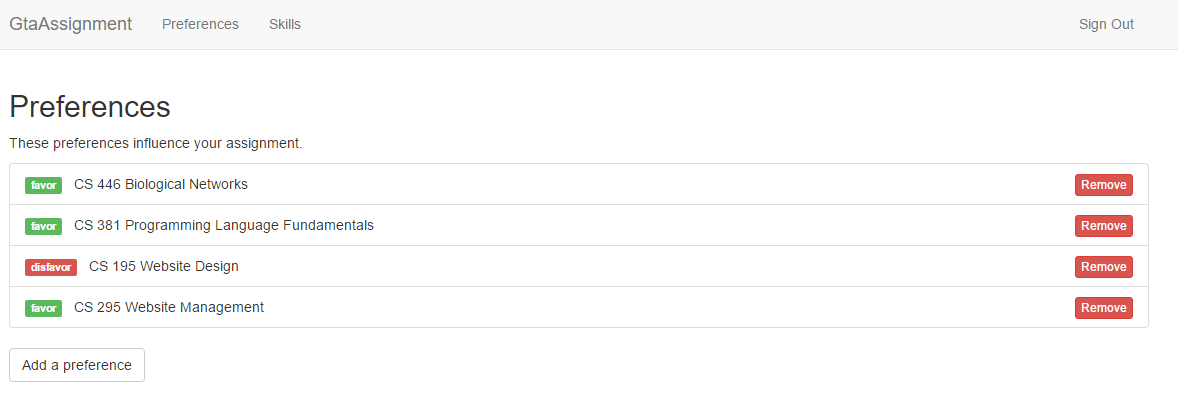
\includegraphics[width=\linewidth]{images/student-preferences-alpha.png}
%     \caption{Mock Student Preferences Interface}
%   \endminipage\hfill
%   \minipage{0.5\textwidth}
%     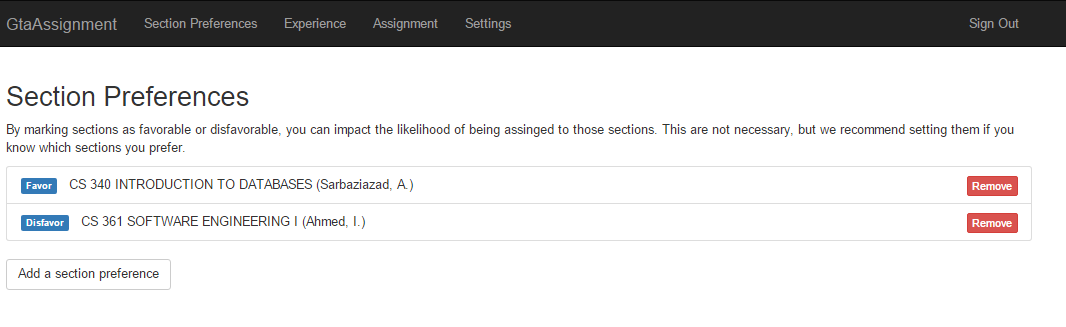
\includegraphics[width=\linewidth]{images/student-preferences-beta.png}
%     \caption{Release Student Preferences Interface}
%   \endminipage\hfill
% \end{figure}

Not a lot has changed from what we envisioned in our mock ups, we added a couple of sentences going into detail about how to use the site along with changing some wording.
We moved away from just preferences to section preferences to show that you are preferring actual sections not just classes.
A class could be taught by multiple instructors each with their own section, so denoting that fact helps clear up some confusion.

Jonah created a web scraper which grabs all the current classes along with course section, instructor, and enrollment sizes.
The list of courses will always be up-to-date because of this.
Students are allowed to select as many preferences as they want.
Each preference has an associated value ranging from Favor to Disfavor with neutral being in the middle.
By default, the section preferences are set to neutral.
This means there is an equal possibility that a student can be assigned any class as long as they have the required skills.
The more preferences they fill out, the greater chance of getting the class they desire.
